\documentclass{article}
\usepackage{graphicx}
\usepackage{color}
\usepackage{mathptmx}
\usepackage{gensymb}
\usepackage{amsmath}
\usepackage{float}
\usepackage{setspace}
\usepackage[top=1in, bottom=1in, left=1in, right=1in]{geometry}
\usepackage{fancyhdr}
\newcommand{\HRule}{\rule{\linewidth}{0.5mm}}
\setlength{\headheight}{15.2pt}
\pagestyle{fancy}


%\pagestyle{myheadings}
\lhead{\bfseries Reentry Experiment SAT-X}
\chead{\textbf{} U. Northern Colorado}
\rhead{\em \today}

\begin{document}
%%%TITLE PAGE%%%
	\begin{titlepage}
		\begin{center}
			% Upper part of the page
			\textsc{\LARGE Un\underline{iversity of Northern Colora}do}\\[0.7cm]
			\textsc{\Large Colorado Space Grant Symposium}\\[0.7cm]
			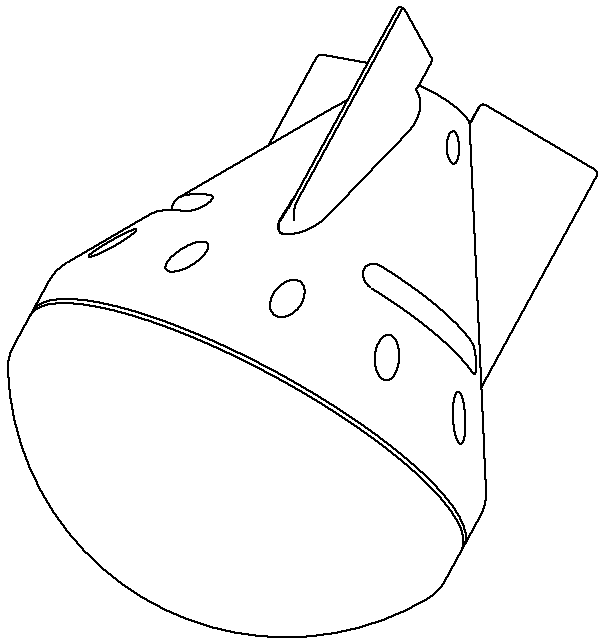
\includegraphics[width=7cm]{CapsuleDrawing}\\[1cm]
			% Title
			\HRule \\[0.4cm]
			{ \huge \bfseries Reentry Experiment SAT-X:\\} \large Developing an Optimal Atmospheric Reentry Vehicle for the Rocket SAT-X Program\\[0.4cm]
			\HRule \\[1.3cm]
			% Author and supervisor
				\begin{minipage}{0.4\textwidth}
					\begin{flushleft} \large
						\emph{Authors:}\\
						Aaron \textsc{Adamson}\\
						Jordan \textsc{Aken}\\
						Motoaki \textsc{Honda}\\
						Casey \textsc{Kuhns}\\
						Rob \textsc{Shiely}\\
						Maurice \textsc{Woods} (PM)
					\end{flushleft}
				\end{minipage}
				\begin{minipage}{0.4\textwidth}
					\begin{flushright} \large
						\emph{Advisors:} \\
						Cynthia \textsc{Galovich}\\
						Matthew \textsc{Semak}\\
						Robert \textsc{Walch}\\
					\end{flushright}
				\end{minipage}
				\vfill
				\vspace{.75cm}
			% Bottom of the page
				\begin{minipage}{0.4\textwidth}
					\begin{flushleft} 
						
\includegraphics[width=2.75cm]{UNC}\\
					\end{flushleft}
				\end{minipage}
				\begin{minipage}{0.4\textwidth}
					\begin{flushright}
						
\includegraphics[width=2.5cm]{NASA}\\
					\end{flushright}
				\end{minipage}

			{\large \today}\\
			Revision 2
		\end{center}
	\end{titlepage}



%%%BEGIN DOCUMENT%%%
\newpage
%Table of Contents
\tableofcontents	
\newpage


%Abstract
\section{Abstract}
	\begin{doublespace}
	\indent\indent The Reentry Experiment SAT-X (ReX), a joint venture between University of Northern Colorado (UNC) Physics and the Colorado Space Grant Consortium (COSGC), was designed to identify key design aspects associated with atmospheric reentry vehicles and to provide test data that will help to remove dependency on over-engineering as a primary engineering strategy. One of the important considerations for space exploration involves the structural challenges experienced by spacecraft upon returning to Earth. The challenge of entering, or reentering, the Earth's atmosphere is not new, and for years NASA has successfully designed vessels that have endured the harsh process of reentry. However, surprisingly little is actually known about the high atmosphere of Earth. With the insight gained from a simple model of a reentry vehicle's interaction with the atmosphere, a variety of prototypes were tested to determine which design stood the best chance of achieving the ReX mission goals. The ReX payload was launched from Wallops Island at NASA's Wallops Flight Facility in Virginia on 21 July 2011. Funded by the COSGC as part of the Rocket SAT-X undergraduate research program, the payload was flown on an Improved Terrier Orion sounding rocket, and it successfully deployed a small aluminum capsule at apogee (at an altitude of approximately 120 km). The flight was intended to function as a means for characterizing the reentry process and as a proof-of-concept test, showing that the capsule design was an effective platform that could be used for further atmospheric research in the Rocket SAT-X program. The payload design was effective at ejecting a vessel from a spacecraft with few moving parts; it can be constructed in less than a month with less than a \$3000 budget, and it is easily modifiable to accommodate new mission hardware (ideal for the Rocket SAT-X program). We are currently revising the ReX design in an attempt to improve the payload's radio telemetry connection, thus increasing the amount of data recovered from the flight and improving the resolution and dependability of the payload's instruments.
	\end{doublespace}

%Introduction
\section{Introduction}
	\begin{doublespace}
		\indent\indent The challenge of entering, or reentering, the Earth's atmosphere is not new. For years, NASA has successfully designed vessels that have endured the harsh process of reentry. However, in some cases, this was made possible through the act of over-engineering; designing to withstand conditions far beyond what is expected to be encountered. Though this method has proven effective, consider the benefit of knowing exactly what to expect. The objective of the University of Northern Colorado Reentry Experiment SAT-X (UNC ReX) was to shed light on the process of atmospheric reentry and provide test data that will help to remove our dependency on over-engineering. Moreover, as a secondary objective, the capsule's design was evaluated to determine its effectiveness in serving as a platform for use in future Rocket SAT-X missions. This evaluation took into account the resources and skills needed to produce the capsule.\\
		\indent This mission was carried out as a part of UNC Physics' involvement with ``Rocket SAT-X", an outreach program funded by the Colorado Space Grant Consortium (COSGC) that presents undergraduate students with an opportunity to become involved in aerospace engineering and the aerospace community at an advanced level. The Rocket SAT-X program challenges students to design and fabricate an experimental payload that will be launched on a Terrier-Orion sounding rocket, provided and launched by NASA's Wallops Flight Facility in Virginia. Four university-made payloads were launched approximately 120km into space, where the rocket then shed its fairing, exposing the payloads to the space environment (Figure~\ref{timeline}). \\
		\indent In an effort to document the methods used throughout this project, this report will discuss both the physics and the engineering behind the reentry experiment for future reentry Rocket SAT-X missions.
	%Mission Statement and Background
	\subsection{Mission Statement and Background}
	\begin{center}
		\emph{To provide a robust design of a deployable and recoverable payload for institutions to use on future Rocket SAT-X missions. With the provision of local data storage, we can greatly increase the amount of data recovered by eliminating the need to transmit restricted amounts of data to the ground.}\\
	\end{center}
		\indent\indent  By collecting extensive dynamical and thermal data as the reentry vehicle enters the earth's atmosphere, ReX aims to provide information on the reentry process of a particular type of vehicle. After reviewing the flight data and comparing it to a mathematical model (outlined in the Methods section) the design of the capsule will be reviewed for its effectiveness as a reentry vehicle. Moreover, this data will be used in refining the model to aid in optimizing the payload design. This analysis will be conducted to the extent that any future Rocket SAT-X team using this capsule platform will be able to predict the details of the capsule's motion (its trajectory and motion about its center of mass), what temperatures will be experienced during flight, and what the general limitations of the capsule platform will be at any given time during a mission.
	%Success Criteria
	\subsection{Success Criteria}
		\indent\indent In order to achieve full `missions success', the ReX payload was required to collect enough usable data at a high enough resolution to create a reliable flight characterization profile for the ReX reentry vehicle. Additionally, this had to be achieved while optimizing the vehicle's mass, size and technological complexity -- a secondary objective to the ReX mission. The resolution needed to create such a profile is determined by the ability of the onboard sensors to detect both large and small deviations in the vehicle's flight path, such as oscillations, high-G accelerations, and turbulence. Also, since extreme heat is characteristic of the reentry process, sensors were required to measure where heat builds up on the vehicle surface. Finally, the payload was designed to survive long enough to allow  data collection until impact (splashdown).\\
		\indent ``Full mission success" would only have been claimed if all of these objectives were met. However, considering the possibility that some objectives may not be met for any reason, levels of ``partial mission success" could be achieved if some of the more basic functions of the payload worked correctly despite the failure of other functions (e.g. if the capsule is ejected but data were not transmitted back to the rocket, then the mission would be considered a ``partial mission objective success").\\
		\indent It is important to note that the mission supervisors at Wallops Flight Facility and the COSGC instated a number of mission requirements beyond those set by the ReX team. Given that the ReX payload involved the ejection of a reentry vehicle that was designed to remain intact throughout descent and splashdown, concern was raised about the possibility of the payload landing in a populated area, presenting a potential hazard to those civilians who may be near a debris fallout area. NASA requires that spacecraft reentry must not exceed a 1:10,000 probability of exposing the ground population to risk (Rochelle, 2004). Therefore, the team was required to ensure that the reentry vehicle would be ejected in a manner that would minimize the risk of becoming a hazard to the ground population. An ejection velocity of no more than $5\frac{m}{s}$ was predicted to keep the capsule within a safe impact radius.
		\end{doublespace}
		
%Methods
\section{Methods}
	\begin{doublespace}
	\indent\indent In an effort to better understand the conditions that would be experienced during the reentry process, the ReX team first studied the fundamental physics of the expected descent. Using a mathematical model, the team optimized the payload's design by building the capsule to specifications that were calculated to enable the capsule to survive the descent from apogee and impact with the ocean.
	%Physics of Reentry
	\subsection{Physics of Reentry}
	\indent\indent Using MATLAB (a technical computing environment), Motoaki Honda developed several programs for use in modeling the flight of the capsule. The programs were to serve three purposes: 1) predict the force of impact that the capsule experiences upon splashdown, 2) predict the amount of energy due to air friction that is imparted to the capsule during its descent (calculate the heat of reentry), and 3) provide a graphical user interface testing tool for visualizing the instantaneous orientation of the capsule during drop tests (also used to ``monitor" the motion of the capsule during flight). The following subsections are an overview of some of the basic concepts that were used in the mathematical model.
		%Forces
		\subsubsection{Forces}
		\indent\indent To model the process of atmospheric reentry, it is important to know what forces are being exerted on the reentry vehicle. Taking a purely Newtonian approach, the most prominent force  associated with reentry is air resistance (Pardini and Anselmo, 2004). This is expressed by
		\begin{equation}
			F_{air drag}=\frac{1}{2}\rho(h) v^{2}AC_{d},
		\end{equation}
		where $\rho$(h) is air density as a function of the altitude, h, above the surface of the earth, $v$ is the capsule's speed, A is the capsule's cross-sectional area, $C_{d}$ is the drag coefficient associated with the capsule's geometry. So, taking this and the force of gravity into account, the capsule's resultant vertical acceleration is given by\\
		\begin{equation}
			a_{resultant}=g(h)-\frac{\rho(h)v^{2}AC_{d}}{2m},
		\end{equation}
		 where g(h) is the altitude-dependent acceleration rate due to gravity and m is the mass of the capsule. Next, recall that g(h) is given by Newton's law of universal gravitation,
 		\begin{equation}
			g(h)=\frac{GM_{earth}}{(R_{earth}+h)^{2}}		
		\end{equation}
		where G is the universal gravitational constant, $M_{earth}$  is the mass of the earth, and $R_{earth}$ is the radius of the earth. With these relations, one can develop the capsule's altitude-dependent speed profile. This is important in what is to come.
		%Air Density
		\subsubsection{Air Density}
		\indent\indent The atmosphere of the earth is not easily describable as there are a great number of variables that cause variations in its composition. As a result, there is no general equation for the density of air with respect to altitude. However, there is information available that describes the atmosphere as a set of layers, each characterized by an average density (Haynes, 2012). Using this data and interpolating with the assumption that the density decays exponentially over each layer, a continuous density profile can be developed by `stitching together' the estimated density profile for each layer (Figure \ref{stitch}).
 		%The 'Atmospheric Wall'
		\subsubsection{The ``Atmospheric Wall"}
		\indent\indent As the ReX capsule descends from space, there is a period of time during which the capsule will effectively be in free fall as drag is negligible. This occurs when the capsule is outside of the earth's atmosphere, which begins at an altitude of roughly 50km (Haynes, 2012). At this altitude, the capsule will experience a sudden increase in atmospheric density. This marks the boundary between a region of virtually infinite terminal velocity to one of significantly lower terminal velocity. Given that that the capsule will have accelerated to a relatively large speed within the free fall region, it will experience a significant deceleration as it crosses this boundary. This sudden deceleration was referred to as ``hitting the atmospheric wall", since the capsule's encounter with the atmosphere is analogous to hitting a wall of air. As the object is dropped from increasingly larger heights, the impact from hitting this `wall' becomes greater (Figure \ref{accel}).
		%Work Done by Air Friction
		\subsubsection{Work Done by Air Friction}
		\indent\indent The capsule's sudden deceleration caused by encountering the `atmospheric wall' can induce not only a large amount of G-shock to the body of the capsule, but also significant heat buildup due to air friction. This became a topic of concern in the design of the payload as both effects could prove hazardous to the functionality of the capsule. In order to estimate the amount of energy involved in heating the capsule, the energy generated by the drag was considered. Using the model for the drag force and the velocity of the capsule throughout its descent (outlined in Section 3.1.1), the magnitude of the power generated due to air drag, $|P|=F_{air drag}v$, was calculated as a function of time. Finally, the power profile was integrated over time to reveal the total energy lost due to drag. This value served as an estimate of the upper bound on the energy that went into heating the capsule (as there was an uncertainty as to how much of this energy was transfered to the atmosphere rather than the capsule) (Figure \ref{heat}).\\
		\indent The mathematical model estimated that more than 2MJ of energy would go into heating the capsule, which would threaten to melt the capsule's aluminum body if the amount of aluminum used to make the capsule was too little. This information led to a side effort to design an ablative heat shield that could be placed over the front of the payload to reduce the amount of thermal energy transfered to the capsule. While this effort was not incorporated into final capsule design, more about the heat shield is included in the ``Payload Design" subsection.\\
		\indent The mathematical model also considered other mechanisms for heat transfer between the capsule and the air. This took into consideration the fact that the air around the capsule would be heated by the capsule itself and what effect this might have on the transfer of energy. Additionally, in the absence of the proper resources to conduct such a test, heating profiles of similarly-shaped spacecraft from other published works were reviewed in order to understand the importance of orienting the reentry vehicle with a stable trajectory so as to prevent imbalances in the heating of the capsule (Pezzella and Viviani, 2011). 

	%Payload Design
	\subsection{Payload Design}
		\indent\indent Based on the mathematical model, there are two aspects of the reentry process that govern the design of the reentry vehicle: thermal loading and sudden changes in velocity (particularly upon landing). By reducing the drag profile of the capsule, the thermal loading on the skin of the vehicle can be significantly reduced. However, by doing this, the resistance to moving through the air is also reduced causing the terminal velocity of the capsule to increase to a level that may cause structural failure upon landing. On the other hand, increasing the drag profile of the capsule reduces the terminal and impact velocities of the falling reentry vehicle but could cause the capsule to overheat due to friction with the atmosphere. Therefore, an appropriate balance between the two hazards must be found.\\
		\indent The ReX team created several prototypes (Figure \ref{proto}) that were used to test the various aspects of flight. While the mathematical model could be used to determine a theoretical value for the terminal velocity and thermal loading for each prototype, additional short range drop tests were also necessary to determine which capsule design was best at orientating itself into a proper, straight-down trajectory (ideally, the capsule would fall nose first without tumbling or high-speed spinning which could cause damage to the internal electronics).  Research involving the development of reentry vehicles by NASA and Boeing suggested that one of the most effective reentry vehicles was the Apollo capsule, used in the 1960's and 70's at the dawn of manned spaceflight (Sietzen, 2011). The Apollo shape features a wide convex disk at its base which created a large drag profile that was structurally supported by the conical shape that was positioned on top of the disk. While this design was promising at first, the team realized that the Apollo capsule was not a freely falling object but was oriented with the help of thrust rockets that could be fired in any direction to maintain a stability about the thrust axis (Cole, 2008). After performing several drop tests, the ``stream-line shaped" capsule (which still retained many of the Apollo spacecraft's basic design features) was deemed to be the most suitable candidate for the final payload design, as the incorporation of tail fins compensated for the lack of rocket-based flight stabilization. Not only did the design orient itself flawlessly during each drop test, but the mathematical model seemed to support the possibility of such a shape surviving the strongest impact of the four designs.\\
		\indent The team then focused on creating a heat shield for the nose of the capsule to prevent overheating and meltdown due to air friction. Due to the intense vibrations and accelerations of launch, ceramics and the more traditionally rigid types of heat shields were deemed inadequate. Instead, the team tested several combinations of carbon fiber and graphite-based epoxies to protect the capsule from the intense heat. A layer of carbon fiber weave, glued on with an epoxy infused with graphite powder, was the most effective means of protecting the capsule (Figure \ref{shield}). However, due to time constraints and difficulties with developing a reliable method for attaching the heat shield to the nose of the capsule, the heat shield was not included in the final payload design.
	%Sub-Systems Overview
	\subsection{Sub-System Overview}
		%Hardware
		\subsubsection{Hardware}
		\indent\indent The ReX payload consisted of one ejectable reentry vehicle that housed an assortment of sensors used to gather dynamical and thermal data during reentry. In addition to the reentry vehicle, the payload was outfitted with a reentry capsule launcher used to jettison the capsule from the rocket body after fairing deployment at rocket apogee.\\
		\indent The exterior housing of the reentry vehicle was designed as a mixture of two `ideal' reentry shapes. As discussed in Section 3.2, the Apollo capsule was chosen as a model for the ReX reentry vehicle. The Apollo capsule's shape provides a great deal of interior space for housing electronics, presents a large, forward-facing surface for heat dissipation, and a low center of gravity that aids in stabilizing the capsule during flight. Additionally, the smooth, conical shape is easily machined, allowing the team to fabricate multiple versions of the same payload for prototyping and testing. However, the Apollo-shape profile alone is not sufficient, as the prototype failed to properly orient itself in a downward-facing `flight trajectory' during testing. To correct for this, the design was modified to incorporate a profile that was more streamlined. With the addition of tail fins to an elongated aft section, the hybrid streamlined-Apollo capsule (Figures \ref{proto} \& \ref{capsule}) exhibited exceptional self-orienting characteristics that will allow the capsule to travel through the earth's atmosphere with minimal tumbling and heating.\\
		\indent  In order to prepare the capsule for a reentry flight, it must be released from the sounding rocket body after the fairing of the rocket has been deployed (Figure \ref{ejection}). To ensure that the capsule is clear of the rocket as it is released, a small spring pushed the capsule from the rocket at approximately $1\frac{m}{s}$ (knowing the expected rotation rate of the rocket, this was the speed required to avoid collisions with any objects protruding from the spinning rocket body). This spring was compressed and placed at the tail of the capsule, which was held in place by a locking mechanism incorporated into the capsule launcher harness. However, to ensure that ejection of the capsule would not occur prematurely, a cylindrical locking cam was designed to lock the capsule in place during launch using positive pressure to ensure that the lock was still engaged regardless of power supply or control systems status (Figure \ref{harness}). When apogee was reached, the motor rotated the cam causing the locks to disengage and release the capsule.\\
		\indent The payload was equipped with multiple microcontrollers, each responsible for collecting data and controlling certain events that must be initiated during the flight. To do this, two main electrical systems were designed, one on the base station and one on the reentry vehicle. Both systems were derived from the ATmega2560 microcontroller and incorporated an array of sensors to completely characterize the three-dimensional motion of the individual components throughout the flight. The sensor equipment included an HMC5843 triple-axis magnetometer, two ADXL345 triple-axis accelerometers, an ITG3200 triple-axis gyroscope, and a LPR530AL dual-axis and LY530AL single-axis gyroscope, all bought from SparkFun Electronics. Additionally, the capsule was designed to carry several temperature sensors to collect data concerning the thermal loads and thermal gradient experienced on the skin of the capsule at different points during the reentry process. However, due to complications with adhering the sensors to the aluminum shell, these temperature sensors were not included in the finished payload.\\
		\indent The base station and capsules communicated via 900MHz radio transceivers. Because these radios were housed within the capsule's aluminum shell, an antenna was necessary to allow the transmission of radio signals to and from the reentry vehicle. To accommodate for this, the tail fins on the tail of the capsule were constructed from printed circuit-board (PCB) that contained a copper trace that would act as an antenna situated outside of the capsule (Figure \ref{antenna}). The antenna's length and shape was designed with the help of First RF in Boulder, CO, who helped the ReX team optimize that antenna's effectiveness.\\
		\indent The base station had several unique functions. It was primarily responsible for receiving and interpreting several timing events from the rocket telemetry. That information was used to activate the subsystems aboard the payload, including a shock resistant, high definition video camera, reentry vehicle electronics, and the launching/capsule release mechanism. The base station also transmitted real-time data and status updates to the launch facility via a telemetry link to the ground, provided by Wallops (Figure \ref{FBD}). The final layout of the ReX payload is pictured in Figure \ref{layout}
		%Software
		\subsubsection{Software} 
		\indent\indent Since the flight included a wide range of acceleration and roll rates that were to be recorded, the gyroscopes and accelerometers operated at different ranges (eg. high/low-G) in order to properly cover the spectrum to be measured. If the high detail, limited range sensors saturated at any point of data collection, the software reverted to the high range sensors, so that neither range nor accuracy would have to be sacrificed. All of the data generated by the sensors was stored locally on non-volatile flash memory cards. The reentry vehicle computer sent an abbreviated, lower resolution copy of the flight data to the base station via 900MHz XBee (DigiKey) radios at 115200 baud. For real-time monitoring (and in case of an unrecoverable payload), the maximum amount of data allowed through the 900MHz connection was transmitted using the rocket's telemetry link to the launch facility.\\
		\indent The base station utilized a series of telemetry and power connections controlled by Wallops Flight Facility to receive timing events from, and transmit data to, the launch facility. The first timing event occurred at T+8 seconds, at which time the base station powered on, ran through the self-diagnostics procedure and initiated a full resolution recording of acceleration and roll rates for the duration of the mission. The last timing event occurred when the fairing was removed from the rocket, to indicate readiness for capsule ejection. 
To transmit data, there were ten parallel lines, each of which was used to indicate the payload's status during the flight. There were also four analog lines utilized by the base station that measured the signal strength of the capsule radio connection. Finally, a single serial connection running at 19200 baud provided summarized segments of the dynamical data transmitted by the capsule throughout the flight. 
	\end{doublespace}
						%%%%Capsule Return Reward%%%%%
						%%%%%Payload Layout (Final Assembly)%%%%	
	%Testing
		%Radio and Sensor Tests
		%Tall Tower
	%Launch and Integration
						%%%%PAYLOAD STACK%%%%
		

%Results
\section{Results}
	\begin{doublespace}
	%Hardware Survival 
	\subsection{Hardware Survival}
		\indent\indent Recovery of the ReX payload after mission termination and splashdown suggested that the capsule was ejected properly at apogee. Successful ejection was confirmed by viewing the onboard video footage of the rocket body and its payloads (Ogg \& Goh, 2011). This showed the capsule leaving the rocket roughly eight seconds after fairing separation, drifting away at a reasonable speed with a nominally stable trajectory. The capsule did not appear to tumble at this time and was oriented so that the nose cone faced the earth (in the direction of descent). The reentry capsule body has  not been recovered. Physical examination of the recovered rocket payload section showed that the payload's computer and electronics box was missing altogether. Evidence of scrapes and buffs in the aluminum deck plate and on the aluminum container of the University of Wyoming's AstroX payload (located directly beneath the ReX payload) suggests that the four M6 bolts that fastened the electronics containment box to the deck plate had been ripped out, allowing the box to detach itself from the rocket. Additionally, the cables that connected the various electronics on the deck plate had been completely severed, not only by the apparent pull of the electronics box as it detached from the rocket, but also from the evidence that the payload underwent so much thermal loading that the rosin-core solder had completely evaporated away. The solder bonded the payload's electrical connections to their respective terminals and the melting of the solder left no bonding agent to connect the wires to the electronics (rosin-core solder has a melting point of about 350\degree C). The evidence of thermal loading was also apparent from the discovery of char marks that streaked across the payload. The heat of reentry, being enough to vaporize solder, burned the plastic off of the Kevlar belt that was used to rotate the locking mechanism of the capsule launcher depositing streaks of black residue on the payload.\\
		\indent The on-board, high-definition video camera and the enclosure in which it was housed (mounted to the deck plate) survived reentry with no adverse effects. However, the SD memory card inside the camera was not functional. Upon inspection, the memory card was corrupted. After dissembling the card, the electrical contacts were throughly cleaned to minimize the damage possibly caused by exposure to seawater. A data recovery program was then utilized to try and obtain any information that may have been stored on the card. This effort proved fruitless, and the only video of the reentry vehicle ejection was provided by CU.
	%Effectiveness of Sensors
	\subsection{Effectiveness of Sensors}
		\indent\indent Telemetry data collected and recorded by Wallops Flight Facility suggested that the ReX payload failed to collect any useful dynamical data from any of the capsule's sensors. The telemetry log showed that the payload's umbilical to the capsule (designed to connect the capsule electronics to the rocket electronics) was operational until capsule separation. After ejection, the capsule's sensors were functional for only six seconds, after which time only intermittent signals were received (Figure \ref{raw}).
		\end{doublespace}

%Discussion
\section{Discussion}
	\begin{doublespace}
		\indent\indent The results of the ReX flight data, both through physical evidence and through interpretation of the data, suggest that the mission was only a partial success. The primary mission objective, to successfully deploy a self-contained capsule from the rocket body, was achieved. The capsule release mechanism opened without incident, the ejection spring accelerated the capsule from the rocket to an optimal speed, no collisions occurred between the ejected capsule and the rocket (i.e., there was no evidence of a ``tip off" -- when the tail fins of the capsule are struck by the rocket, causing the capsule to tumble), and video footage of the ejection was acquired for the entire time that the capsule was visible. However, for all practical purposes, the mission did not yield any quantifiable data from the sensors housed on the rocket nor within the reentry capsule. This was due to the fact that there was a fatal error that occurred with the radio connection between the capsule and the rocket payload, as the telemetry data recorded less than ten seconds of data. Any data that were collected during the flight and recorded on the SD card housed within the electronics containment box was lost when the electronics box was ripped off of the deck plate -- no ``hard data" were collected from the flight. However, it is worth mentioning that the char marks on the deck plate left an outline around what was once the electronics containment box. This suggests that the ejection of the electronics box occurred well after the capsule's deployment, therefore ruling out the theory that the lost data connection indicated on the telemetry log was due to a physical failure. Instead, it was due to an error within the electronics/radio system. Unfortunately, without the electronics containment box and without sufficient telemetry data, the ReX team has been unable to diagnose the issues of the flight any further. However, lessons can be learned from the study of the hardware that was recovered from the flight.
	\end{doublespace}

%Conclusions
\section{Conclusions}
	\begin{doublespace}
		\indent\indent The ReX mission was considered a ``partial mission success", based on the \emph{Success Criteria}. While the electronics of the payload failed for unknown reasons, the mechanical system successfully deployed the reentry capsule from the rocket. Even so, it is obvious that the ReX payload contained several design flaws that are now understood from the de-integration of the payload post-flight. Future missions will require the use of RTV (Room-temperature vulcanization), a non-conductive, silicone-based rubber that is used to insulate solder joints from extreme heat and corrosion. Using RTV may have prevented the vaporization of the solder joints that connected the payload's wires to the various electrical components within the electronics containment box, potentially extending the lifetime of the data-collection systems. Furthermore, the absence of the electronics containment box post-flight suggested that the hardware that was used to restrain the box was insufficient or faulty. The helicoils (threaded inserts used to give holes drilled in soft metals a threaded finish, allowing for the use of bolts and screws) that held the M6 bolts to the deck plate had been ripped out. This may be prevented in the future by using more than four bolts to restrain mechanisms to the deck plate.\\
		\indent Of course, the true limiting factor in the design and manufacturing processes of the ReX mission was time. While the team put many hours into constructing the payload, the mission goals were more ambitious than initially anticipated. However, it is reasonable to consider the 2011 Rosanova 41.029 flight as a first trial for an ambitious project to be improved and expanded.
	\end{doublespace}
	%Future Refinement (RAPTR SAT-X)
%	\emph{Future Missions (RAPTR SAT-X)}\\
%		\indent RAPTR
	%Contributions to NASA
	\subsection{Contributions to NASA}
	\begin{doublespace}
		\indent\indent The secondary objective of this project was to utilize the ReX team's unique skill set and hardware access to be able to design a generic platform that COSGC would be able to offer to other schools that may not have the resources of the ReX team. By developing a tested platform to carry and eject payloads into space, future deployable-based university payloads would be able to spend more time on the science of the project, rather than spending time developing the vehicle used to carry and eject it. The ReX capsule, complete with design diagrams and relatively simple manufacturing, makes the possibility of space experiments much less intimidating when a major portion of the engineering has already been completed and tested.  This objective was achieved as the launch mechanism functioned properly, and the capsule was safely ejected and reentered the atmosphere.
	\end{doublespace}

\newpage
%Acknowledgments
\section{Acknowledgments}
	\begin{doublespace}
		\indent\indent The five members of the Reentry Experiment SAT-X team spent a full year designing, testing, perfecting, launching, and analyzing the small piece of aluminum that would be each member's "first item in space". While each member devoted ample amounts of time to see the ReX mission to its completion, ReX would not have been as successful as it was had it not been for the many people that helped along the way. Special thanks is due to Dr. Cynthia Galovich, Dr. Matthew Semak, and Dr. Robert Walch (physics professors at the University of Northern Colorado), and Ken Cochran and Chad Wangeline (technical staff members at UNC) for their advice and support. Also, two companies, Road Narrows Robotics of Loveland, CO and First RF of Boulder, CO, were instrumental in providing workspace and radio-engineering advice. Finally, the advising bodies at the Colorado Space Grant Consortium (particularly mission manager, Shawn Carroll) and NASA's Wallops Flight Facility were extremely helpful and were an invaluable resource to the ReX team.\\
		\indent A web-page containing pictures and videos of the ReX project is located at the following URL:\\ \textcolor{blue}{http://www.facebook.com/pages/University-of-Northern-Colorado-Rocket-SAT/162201893803346}.\\ The ReX team invites you to review the page to keep up with future UNC rocket missions.
	\end{doublespace}

%Literature Cited
\section{Literature Cited}
	\begin{doublespace}
Cole, E. G. (2008). DESIGN AND DEVELOPMENT OF THE APOLLO THREE-MAN SPACECRAFT WITH\\
\indent TWO-MAN LUNAR EXCURSION MODULE (LEM). Annals of the New York Academy of Sciences, 134(1),\\
\indent 39-57. doi:10.1111/j.1749-6632.1965.tb56141.x\\
Ogg, C. (Designer), \& Goh, A. (Designer) (2011). Rosanova 41.092 onboard payload survalence [DVD].\\
Pardini, C., \& Anselmo, L. (2004). On the accuracy of satellite reentry predictions. Advances in Space Research,\\ \indent 34(5), 1038-1043. doi:10.1016/j.asr.2003.01.010\\
Pezzella, G., \& Viviani, A. (2011). Aerodynamic analysis of a mars exploration manned capsule. Acta\\
\indent Astronautica, 69(11), 975-986. doi:10.1016/j.actaastro.2011.06.020\\
Rochelle, W. C., Marichalar, J. J., \& Johnson, N. L. (2004). Analysis of reentry survivability of UARS spacecraft.\\ \indent Advances in Space Research, 34(5), 1049-1054. doi:10.1016/j.asr.2003.01.011\\
Sietzen Jr. (2011). Son of apollo: A new space capsule takes shape. Aerospace America, 49(1), 36.\\
Sim, H., \& Kim, K. (2011). Reentry survival analysis of tumbling metallic hollow cylinder. Advances in Space\\ 
\indent Research, 48(5), 914-922. doi:10.1016/j.asr.2011.04.036\\
U.s. standard atmosphere. In (2012). W. Haynes (Ed.), \emph{CRC Handbook of Chemistry and Physics} (pp. 555-999).\\ \indent Retrieved from http://www.hbcpnetbase.com/

	\end{doublespace}
	
%Figures
\newpage
\section{Figures}
	\begin{figure}[h]
	\begin{center}
		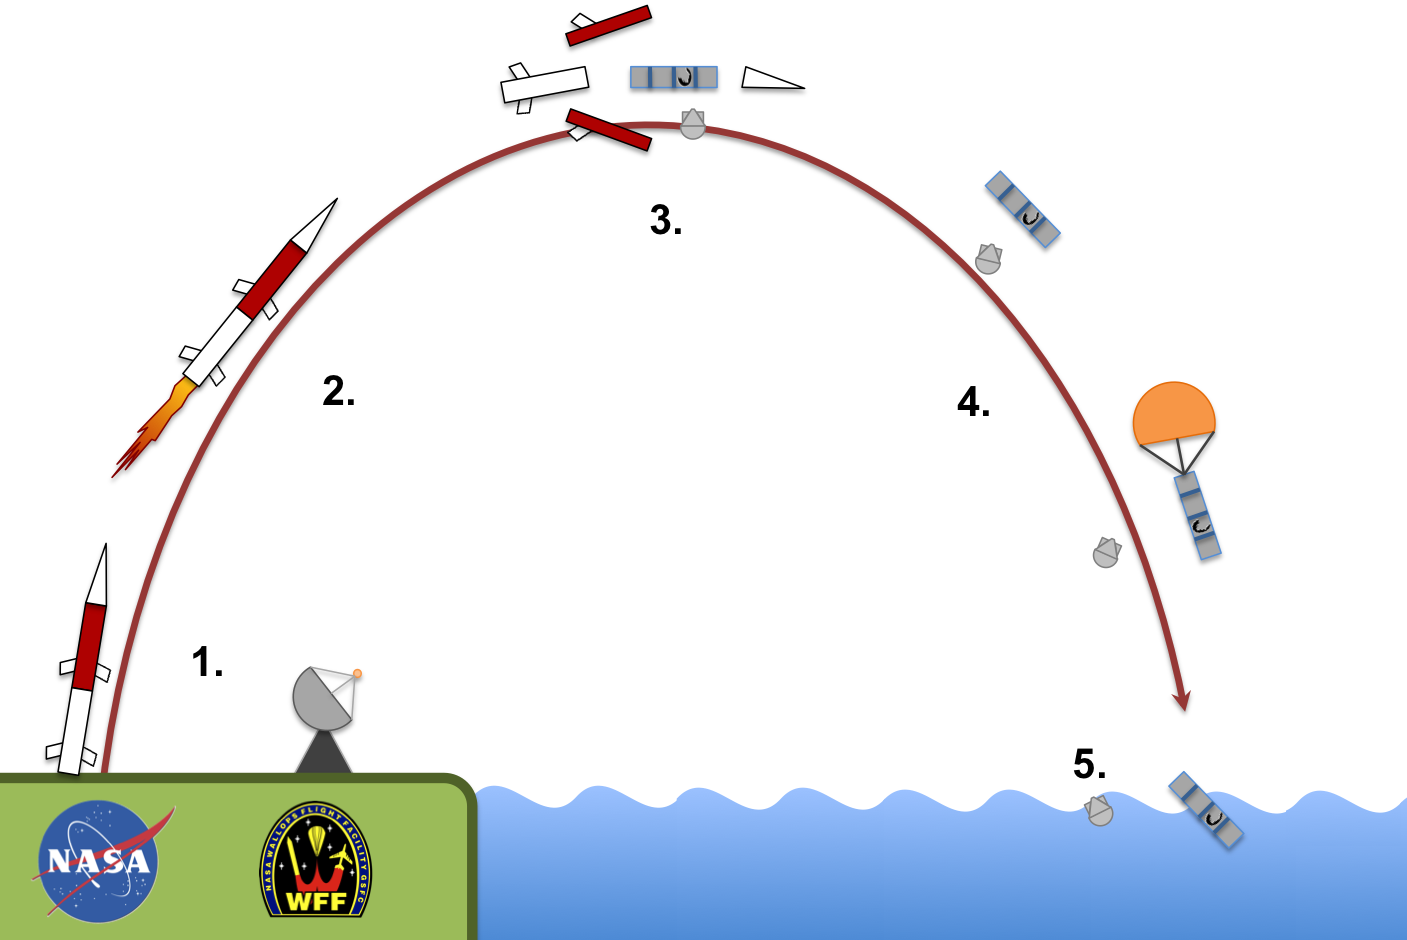
\includegraphics[width=10cm]{ConceptOfFlight}\\
	\end{center}
		\caption{}
		\label{timeline}
Concept of flight timeline\\1. Launch,  2. Ascent; Onboard electronics initialize,  3. Apogee; Fairing deployment, ReX capsules ejected,  4. Descent; ReX Capsules collect data, data transferred via XBee radio to rocket then to ground via Wallops telemetry connection,  5. Splashdown.
	\end{figure}

	\begin{figure}[H]
	\begin{center}
		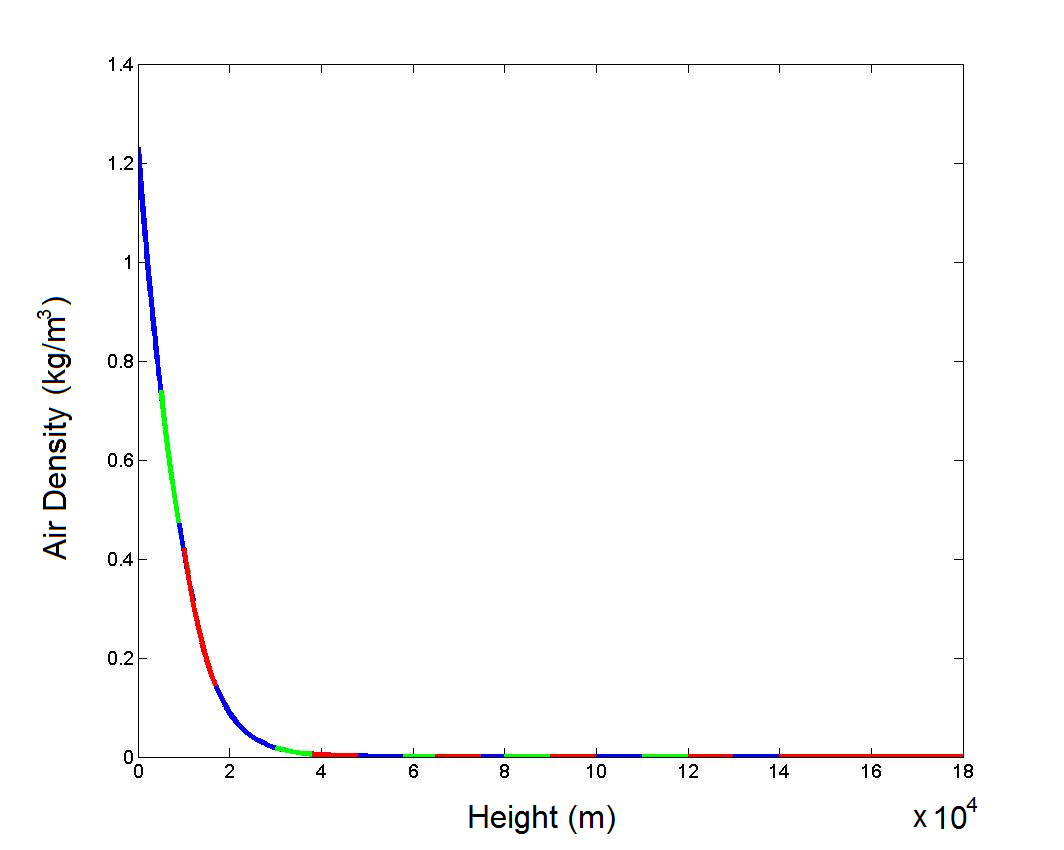
\includegraphics[width=10cm]{StitchedAirDensity}\\
	\end{center}
		\caption{}
		\label{stitch} 
The continuous atmospheric density profile\\ This profile was constructed by stitching together the estimated density profile for each layer of the atmosphere for use in the mathematical model (Haynes, 2012). Each color represents a layer of the atmosphere for which the density profile was estimated.
	\end{figure}
	
\newpage
	\begin{figure}[H]
	\begin{center}
		(A.)
		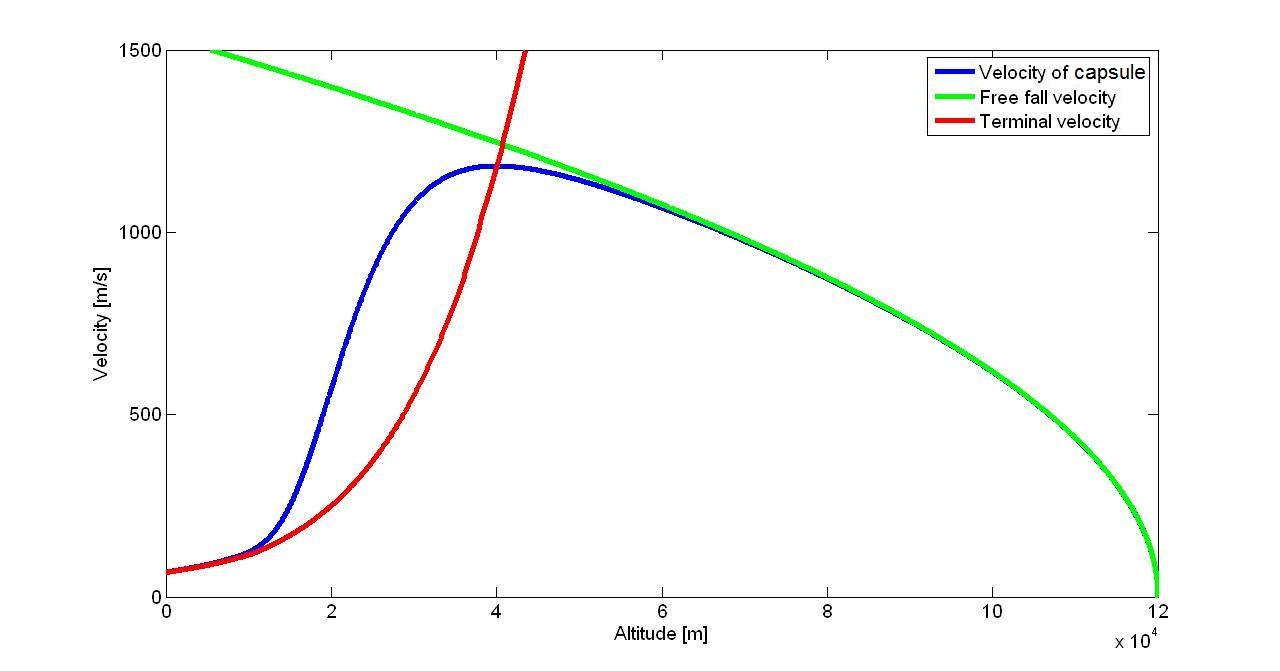
\includegraphics[width=14cm]{BallDrop_120km}\\
		\vspace{1cm}
		(B.)
		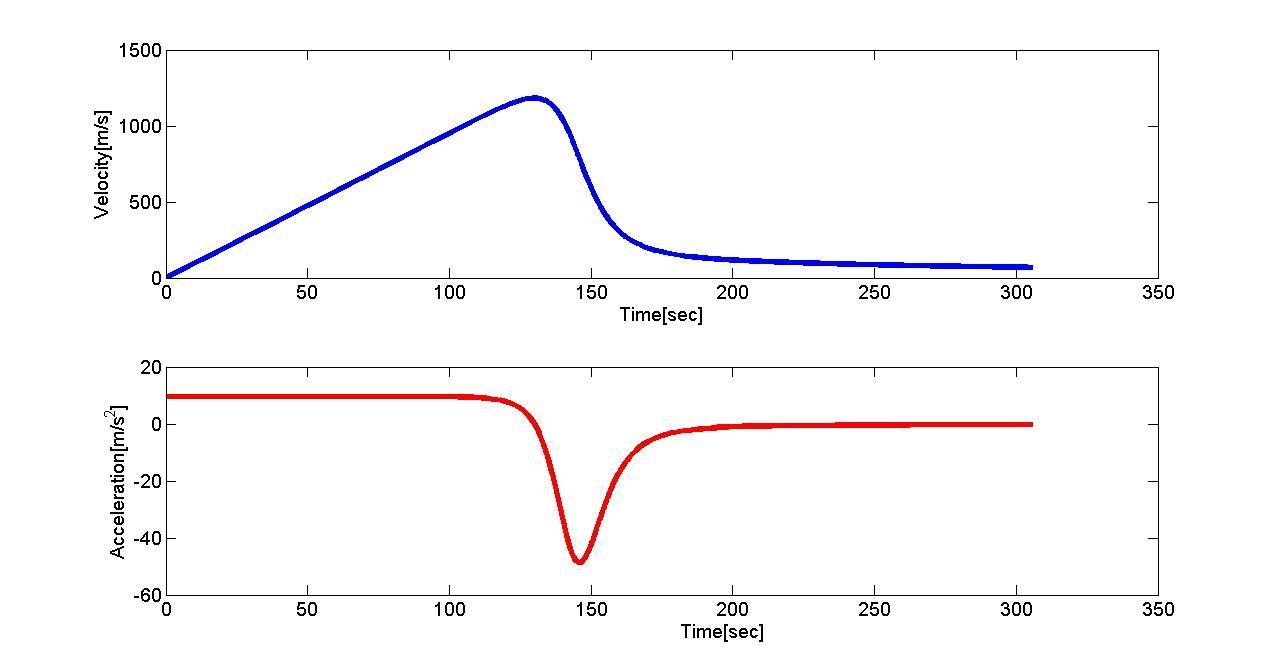
\includegraphics[width=14cm]{KinematicsBallDrop_120km}\\
	\end{center}
		\caption{}
		\label{accel}
Expected velocity and acceleration profiles of the capsule during reentry\\ (A) This velocity profile shows the point at which the capsule is expected to deviate from a free fall trajectory to one with considerable drag. The green curve represents a purely free fall scenario, whereas the blue curve is the expected trajectory that includes the effects of both gravity and air resistance. The red curve is the terminal velocity corresponding to the motion profile of the blue curve. Notice: Where the green and blue curves coincide is the range of altitudes over which the capsule is freely falling, where as the point at which the blue and green curves deviate is the altitude at which the capsule encounters a sudden increase in atmospheric density (ie. ``hits the atmospheric wall"). As seen by examining the red curve, the capsule's speed is higher than its expected terminal velocity for a considerable portion of the flight though the higher-density region.\\ (B) This specific velocity/acceleration profile shows the large negative acceleration experienced in hitting the atmospheric wall.
	\end{figure}

\newpage
	\begin{figure}[H]
	\begin{center}
		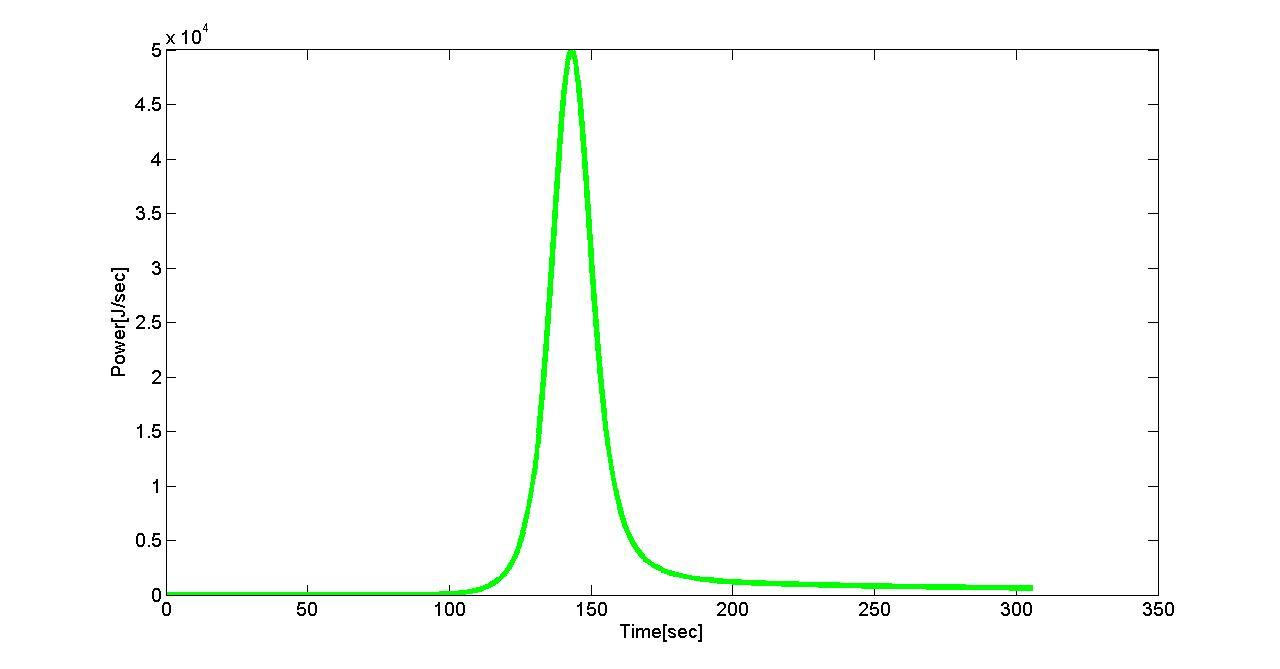
\includegraphics[width=14cm]{ThermalTransfer}\\
	\end{center}
		\caption{}
		\label{heat}
Thermal energy of reentry\\ \indent This is the power generated due to the drag force opposing the capsule's motion through the denser regions of the atmopshere. The area beneath the curve corresponds to the total work done by air friction, which will be transferred into heating up the surface of the reentry object.
	\end{figure}

	\begin{figure}[H]
	\begin{center}
		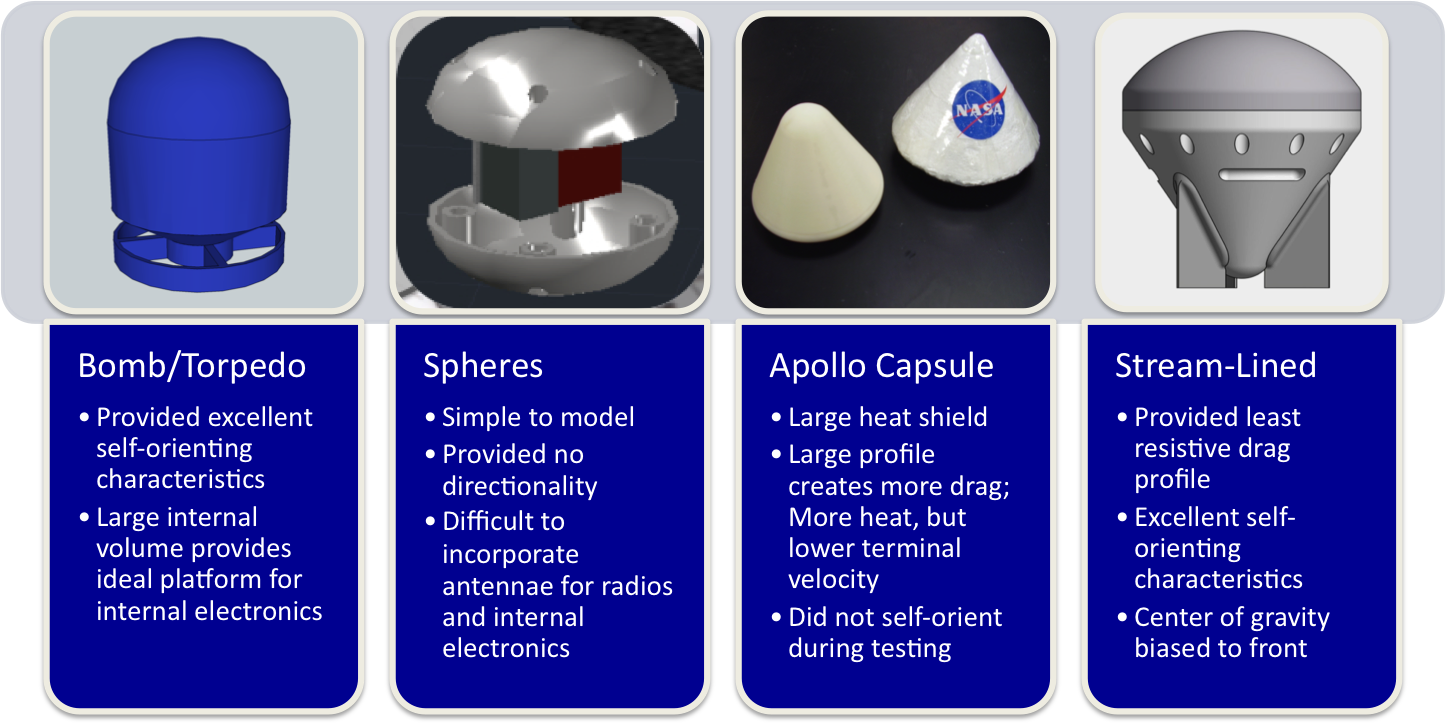
\includegraphics[width=14cm]{Prototypes}\\
	\end{center}
		\caption{}
		\label{proto}
Capsule prototypes\\ Four prototype concepts for the ejectable reentry capsule. The stream-lined shape (an elongated version of the Apollo capsule with tail fins) was decided to be the most appropriate shape for the final reentry vehicle.
	\end{figure}

\newpage
	\begin{figure}[H]
	\begin{center}
		(A.)
		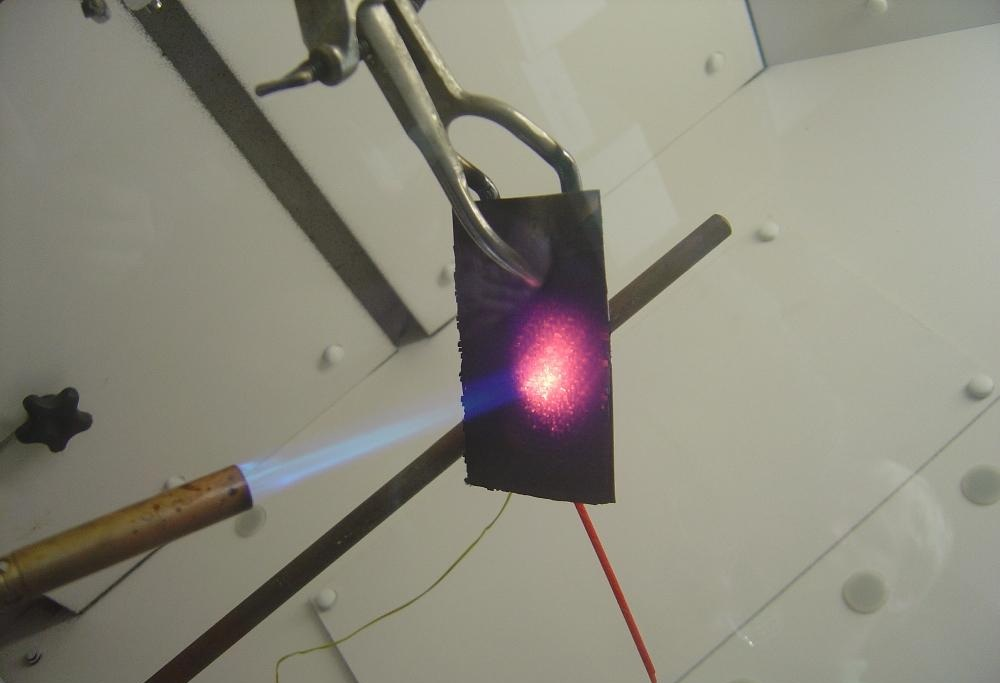
\includegraphics[width=11cm]{HeatShieldTest}\\
		\vspace{1cm}
		(B.)
		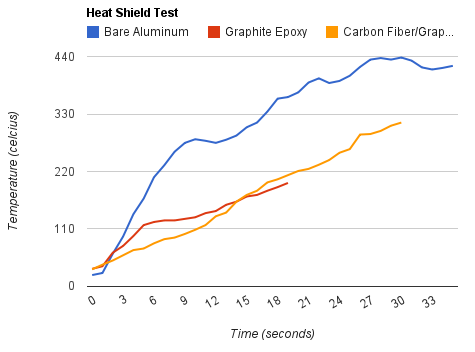
\includegraphics[width=11cm]{HeatShieldTemperatures}\\
	\end{center}
		\caption{}
		\label{shield}
Heat shield development\\(A) An image of the heat shield testing setup: sheets of aluminum were suspended over a butane torch flame for several seconds. Temperature probes were attached to the back of each sheet while the aluminum was heated which recorded the temperature of the back-side of the aluminum every five seconds. \\(B) Average temperature data from three trials of three heat shield types: Bare Aluminum (control/no heat shield), graphite epoxy (an epoxy paste mixed with graphite powder that was smeared over the face of the aluminum and allowed to dry), and carbon fiber weave that was glued to the aluminum using the graphite epoxy paste. Trials were conducted until a relative equilibrium was reached or until a catastrophic failure of the aluminum occurred. 
	\end{figure}

\newpage
	\begin{figure}[H]
	\begin{center}
		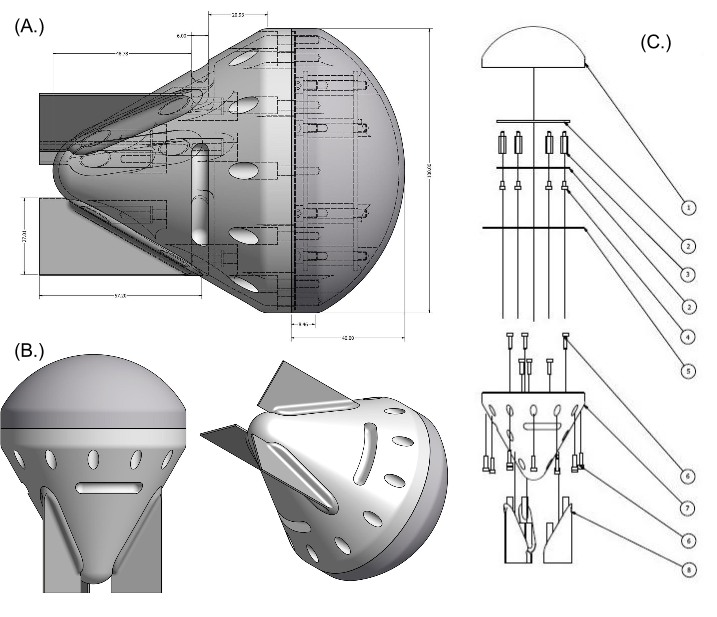
\includegraphics[width=11.5cm]{CapsuleCAD}\\
	\end{center}
		\caption{}
		\label{capsule}
Digital model of reentry capsule\\ (A) Cross-sectioned dimensional view. \\(B) Side and isometric view. \\(C) Exploded view with labeled components: 1. Nose Cone, 2. Electronics deck, 3. Standoff, 4. Nose bolt, 5. Junction Gasket, 6. Junction bolt, 7. Tail, 8. Tail fin.
	\end{figure}
	
	\begin{figure}[H]
	\begin{center}
		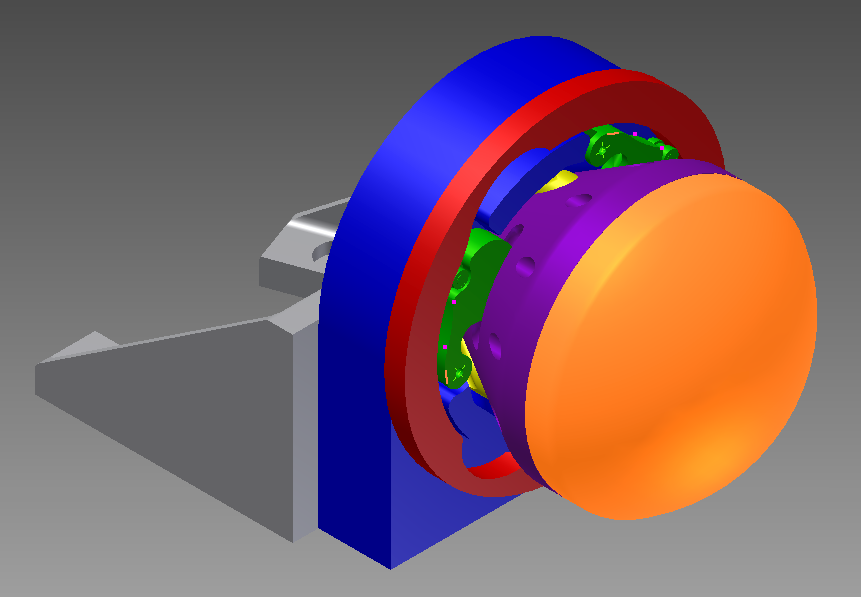
\includegraphics[height=5cm]{HarnessLaunch1}
		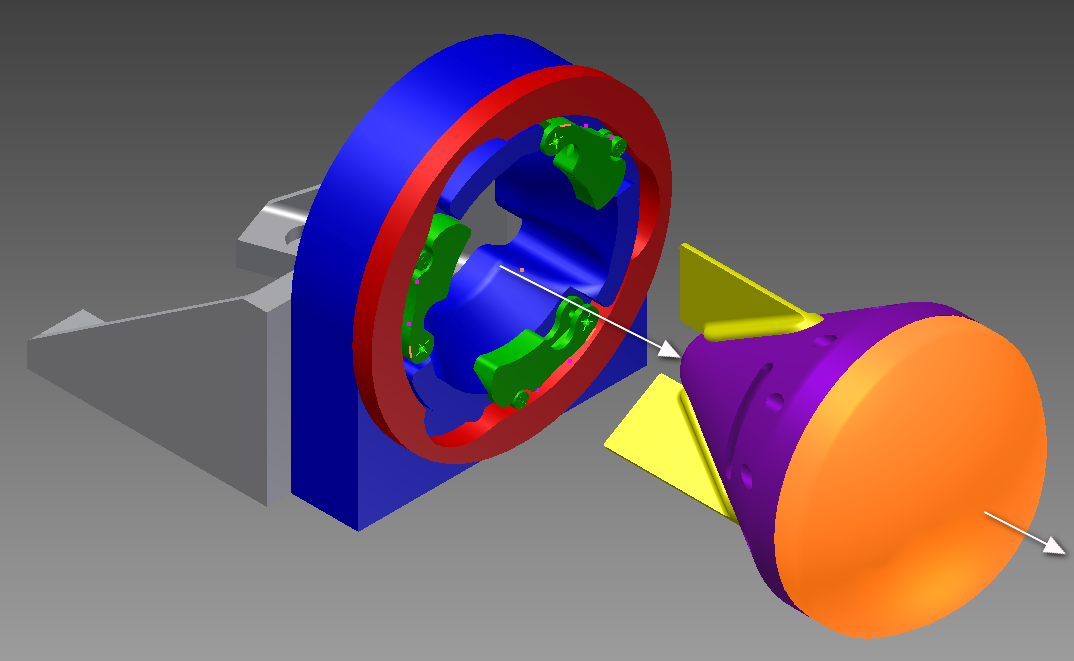
\includegraphics[height=5cm]{HarnessLaunch2}\\
	\end{center}
		\caption{}
		\label{ejection}
Capsule ejection sequence\\ The capsule (purple/orange) is held within the harness (blue) and secured by the latches (green). When the ejection sequence is initiated, the cam (red) rotates to allow the latches to release the capsule, allowing the spring (not visible) to push the capsule out of the harness.
	\end{figure}

\newpage
	\begin{figure}[H]
	\begin{center}
		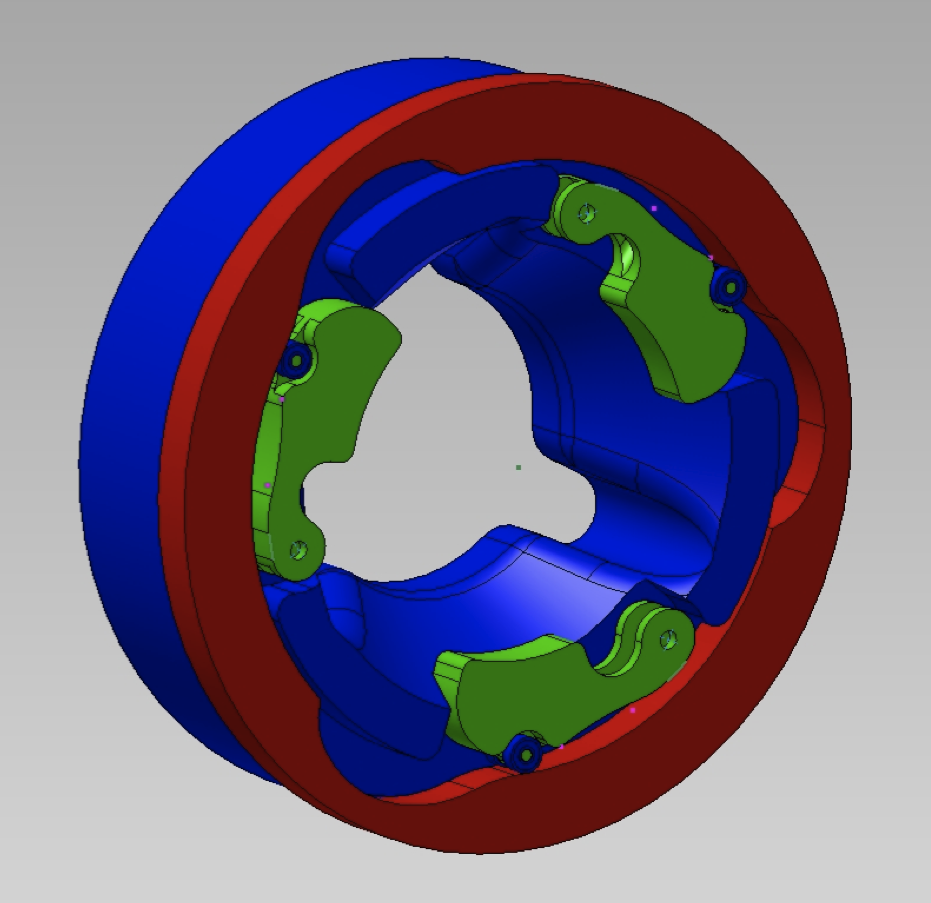
\includegraphics[width=7.7cm]{HarnessCAD}\\
	\end{center}
		\caption{}
		\label{harness}
Capsule harness/locking system\\ The shape of the capsule harness' (blue) interior is the negative of a cone, and cradles the capsule's tail and tail fins. The latches (green) slide into the slots located on the side of the capsule's tail, allowing the latches to lock the capsule in place within the harness. To release the capsule, the cam (red) rotates to allow the latches to hinge outward. The latches are spring-loaded, and so they are forced outward, releasing the capsule. (Refer to Figure \ref{capsule} for information on the capsule)
	\end{figure}

	\begin{figure}[H]
	\begin{center}
		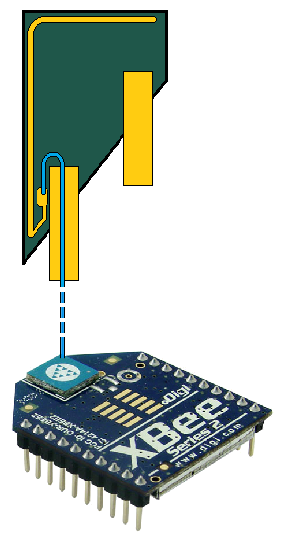
\includegraphics[height=7.7cm]{Antenna1}\hspace{1cm}
		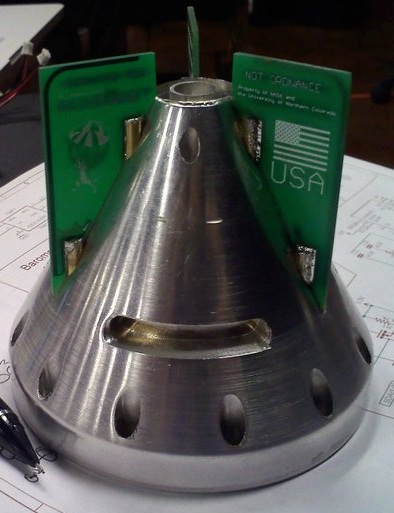
\includegraphics[height=7.7cm]{Antenna2}\\
	\end{center}
		\caption{}
		\label{antenna}
Tail fin antenna\\ The tail fins on the tail of the capsule were made of printed circuit board. Printed on the tail fin was a thin copper trace that was connected to a XBee radio within the capsule shell. The trace was cut down to a size that optimized signal transmission.
	\end{figure}


\newpage
	\begin{figure}[H]
	\begin{center}
		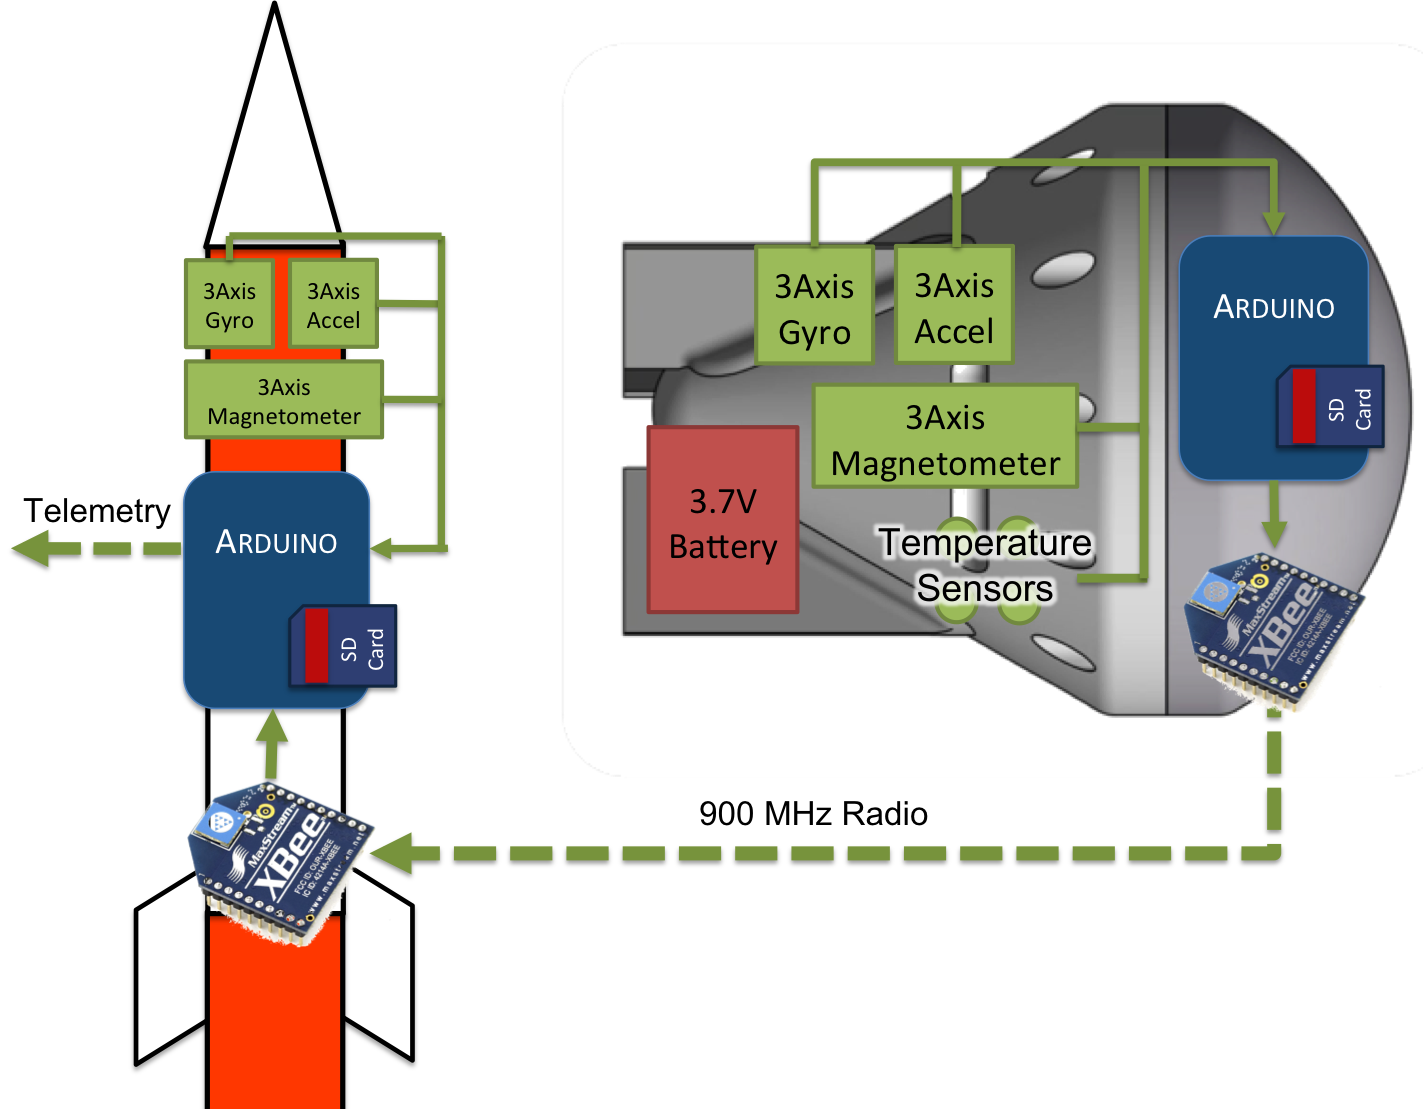
\includegraphics[width=10.5cm]{FunctionalBlockDiagram}\\
	\end{center}
		\caption{}
		\label{FBD}
Functional block diagram of the payload's electronics\\ This diagram includes the basic concept of operations for the payload's power distribution and data transfer along with the sensors and computers used to regulate the transfer of data.
	\end{figure}

	\begin{figure}[H]
	\begin{align*}
		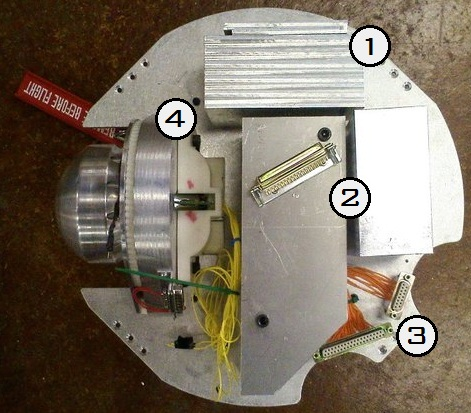
\includegraphics[height=7cm]{Layout2}&&\hspace{1cm}
		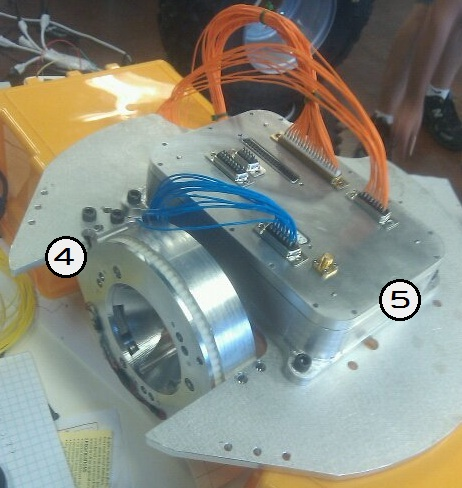
\includegraphics[height=7cm]{Layout1}\\
		Top~Side & &Bottom~Side
	\end{align*}
		\caption{}
		\label{layout}
Payload layout\\ The top side (facing toward the nose of the rocket) of the payload holds the GoPro camera box (1), mass ballast (2), the power/telemetry interface to the rocket (3), and the capsule harness (4) (the white plastic behind the harness houses the ejection spring and capsule umbilical). The bottom side holds the electronics box (5).
	\end{figure}

\newpage
	\begin{figure}[H]
	\begin{center}
		(A.)
		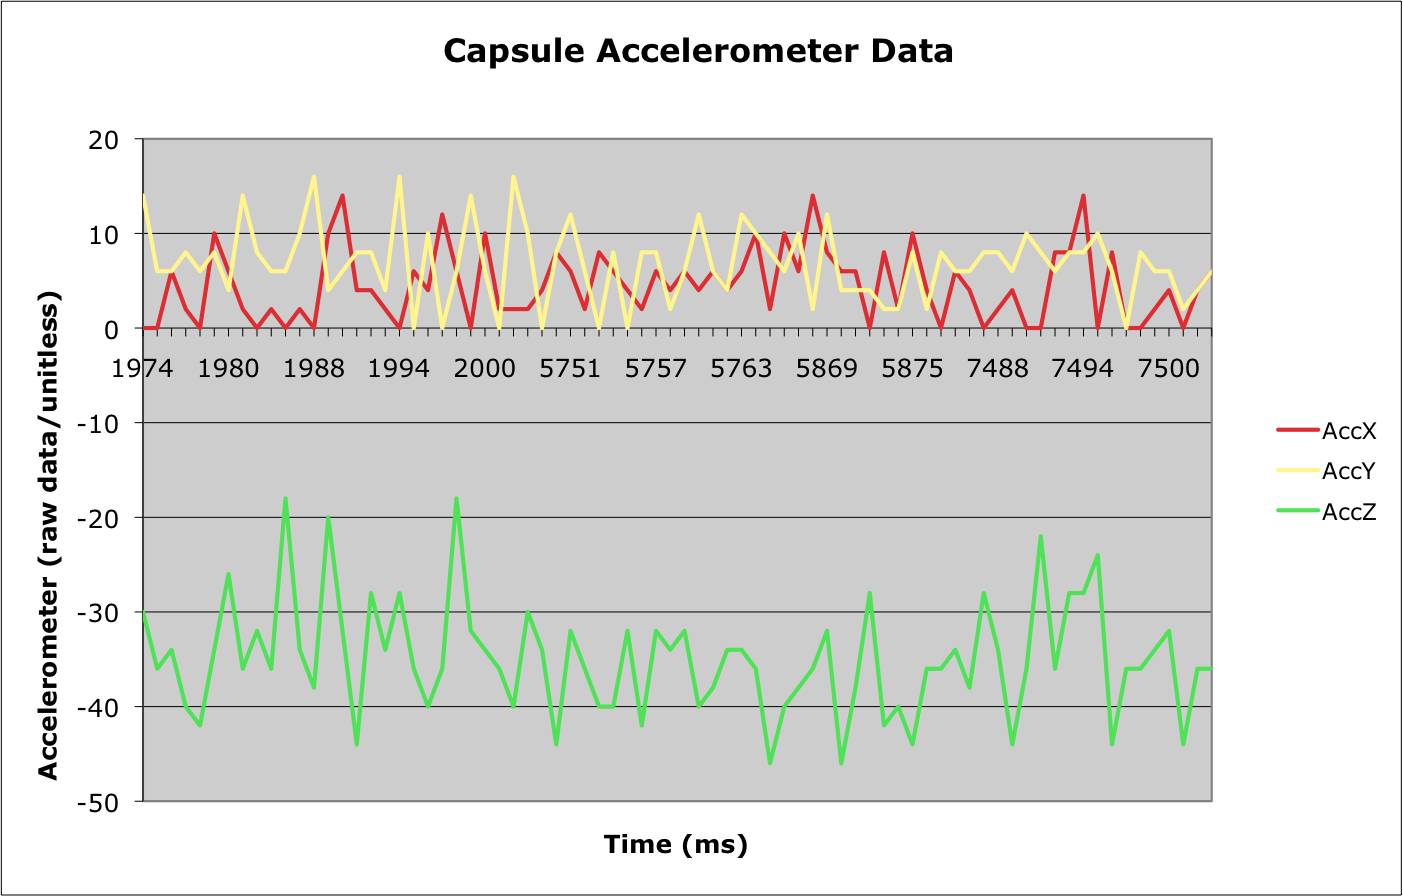
\includegraphics[width=9.7cm]{RawAccel}\\
		(B.)
		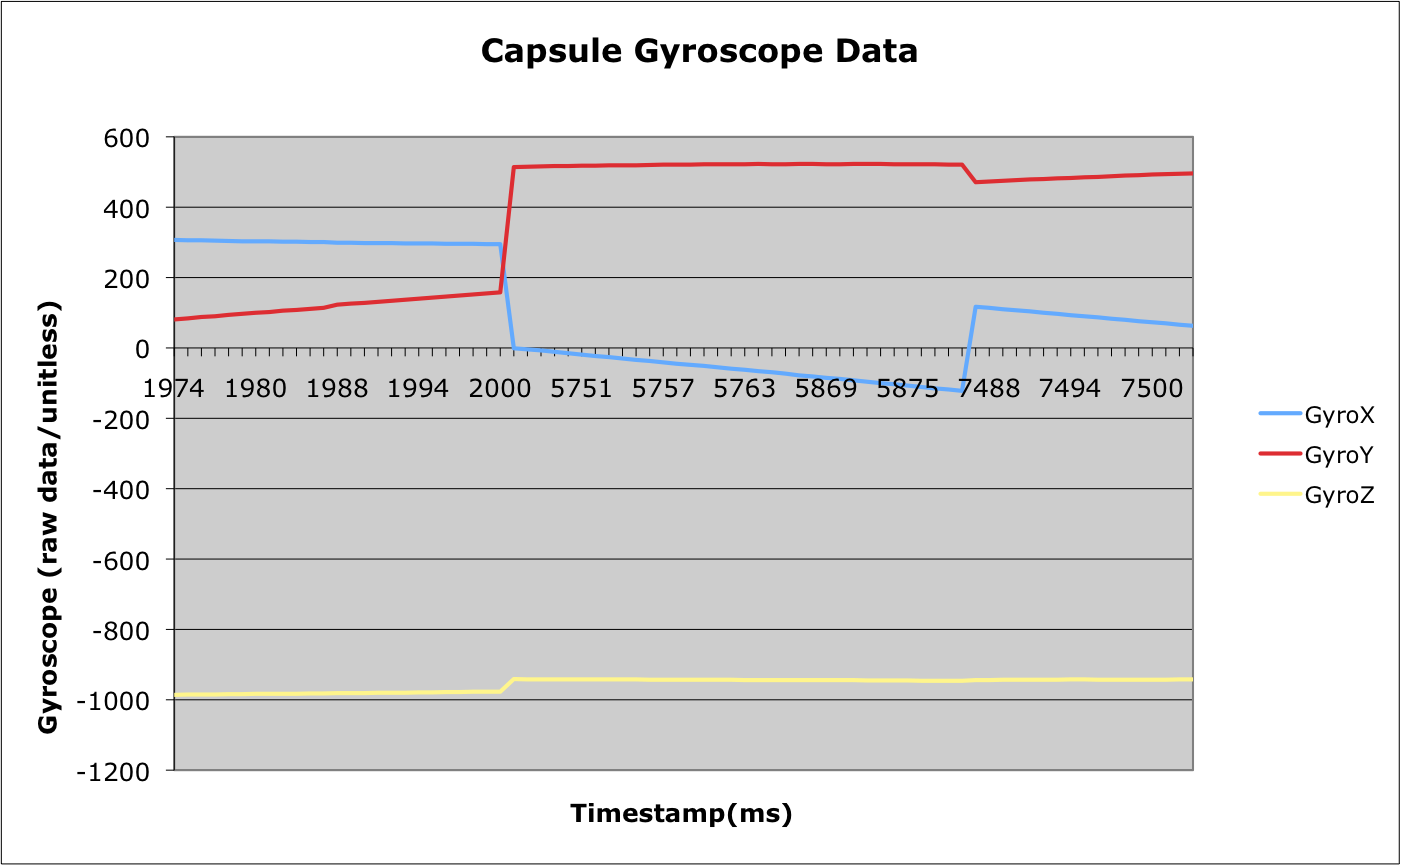
\includegraphics[width=9.7cm]{RawGyro}\\
		(C.)
		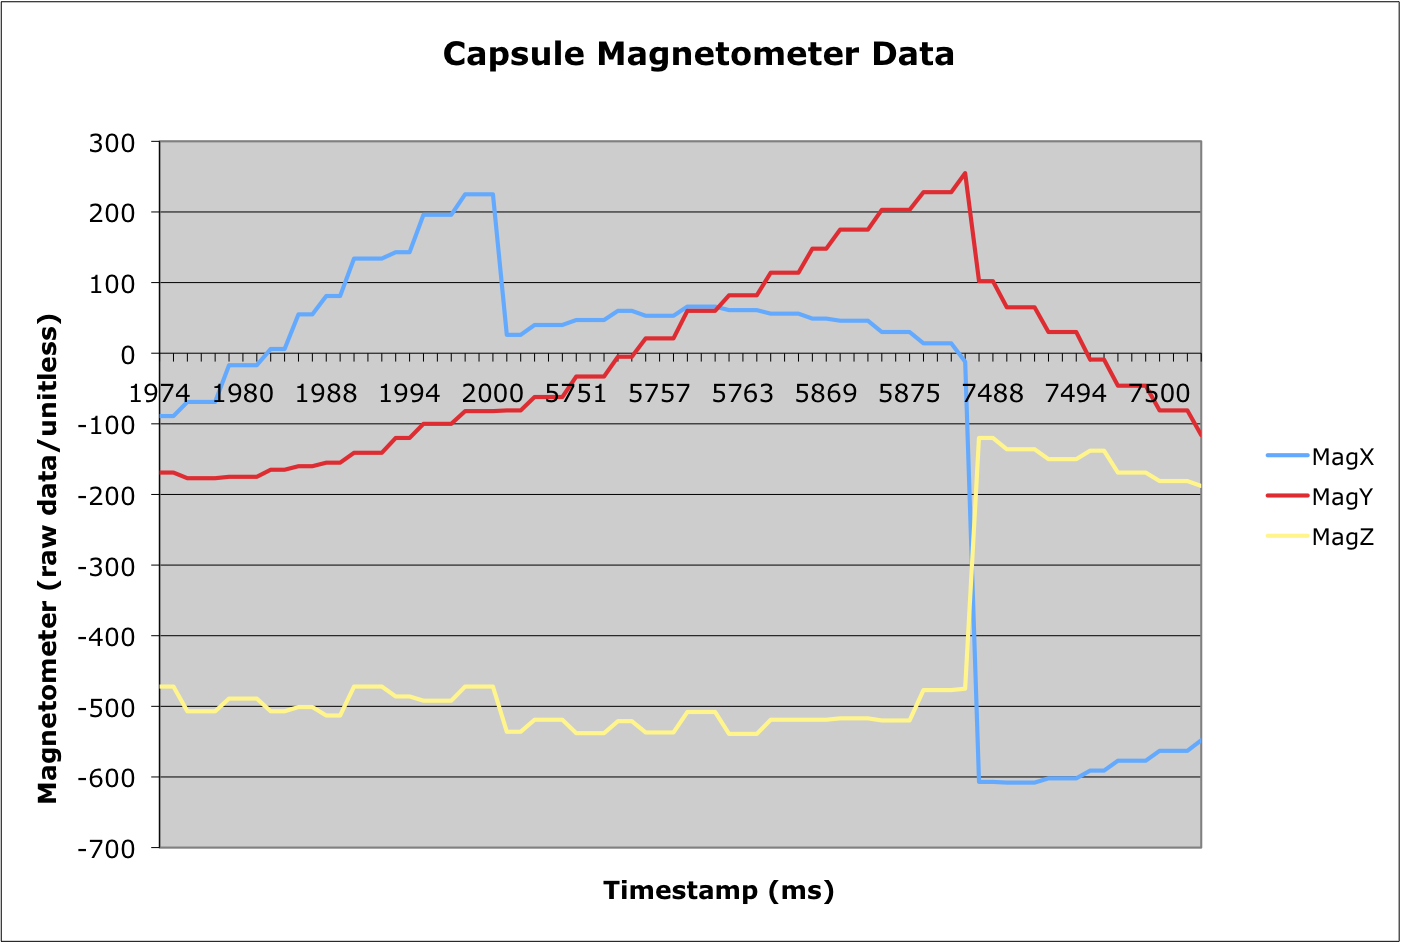
\includegraphics[width=9.7cm]{RawMag}\\
	\end{center}
		\caption{}
		\label{raw}
Recovered flight data\\ The above plots are IMU sensor data from the capsule. The plots show the same time interval (approximately 6 seconds long) which was recorded immediately following fairing ejection/capsule initialization. While the accelerometer data (A) does not present any noticeable trends, it is interesting to note that there are significant events that occur in plots B and C at time +2s and +7.5s. This suggests that the sensors were recording physical movement of some kind, although not enough information was gathered to accurately determine what event this might signify.
	\end{figure}
\newpage

\end{document}